%%%%%%%%%%%%%%%%%%%%%%%%%%%%%%%
\newif\ifPROF

%\def\PourProf{0}
\ifdefined\PourProf
  \PROFtrue
  \newenvironment{corr}{\begingroup \color{blue}}{\normalcolor \endgroup}
\else
  \PROFfalse
  \newenvironment{corr}{\begingroup \color{white}}{\normalcolor \endgroup}
\fi
%\PROFtrue

%%%%%%%%%%%%%%%%%%%%%%%%%%%%%%%%%%%%
\documentclass[12pt, handout]{beamer}
\usepackage{tikz}
%\useoutertheme[left,height=0pt,width=0.12\paperwidth]{sidebar}
%\setbeamertemplate{sidebar canvas left}[vertical shading][top=blue!50, bottom=black!5!black]

\usetheme{Madrid} 


\setbeamercolor{frametitle}{fg=white,bg=blue!50}
\setbeamercolor{background canvas}{bg=purple!8}

%\addtobeamertemplate{footline}
%{%
%   \usebeamercolor[fg]{author in sidebar}
%   \vskip-1cm\hskip10pt
%   \insertframenumber\,/\,\inserttotalframenumber\kern1em\vskip2pt%
%}



\newcount\total
\newcount\lasttotal
\newcount\targetbase

%%%%%%%%%%%%%%%%%%%%%%%%%%%%%%%%%%%%%%%%%%%%%
\usepackage[framemethod=tikz]{mdframed}
\usepackage{tikz, xcolor, lipsum}
\makeatletter
\mdfsetup{skipabove=\topskip,skipbelow=\topskip}

\tikzset{titre_bleu_snir/.style =
	{draw=bleu_snir, line width=1.5pt, fill=white,
	rectangle, rounded corners, right,minimum height=2em}}
\newcommand{\titreencadre}{Titre}
\makeatletter
\mdfdefinestyle{encadrestyle}{%
	linewidth=1.5pt,roundcorner=5pt,linecolor=bleu_snir,
	apptotikzsetting={\tikzset{mdfbackground/.append style ={%
		fill=white}}},
	frametitlefont=\bfseries,
	singleextra={%
		\node[titre_bleu_snir,xshift=2em] at (P-|O) %
			{~\mdf@frametitlefont{\titreencadre}\hbox{~}};},
	firstextra={%
		\node[titre_bleu_snir,xshift=2em] at (P-|O) %
		{~\mdf@frametitlefont{\titreencadre}\hbox{~}};},
	}
\mdfdefinestyle{encadresanstitrestyle}{%
	linewidth=1.5pt,roundcorner=5pt,linecolor=bleu_snir
	apptotikzsetting={\tikzset{mdfbackground/.append style ={%
		fill=yellow!20}}},
	}

\newenvironment{encadre}[1]{\renewcommand{\titreencadre}{#1}
	\begin{mdframed}[style=encadrestyle]
	\vspace{0.5\baselineskip}
	}{%
	\end{mdframed}}

\newenvironment{encadresanstitre}{
	\begin{mdframed}[style=encadresanstitrestyle]
	}{%
	\end{mdframed}}
\makeatother
\usepackage{colortbl}
\definecolor{vert_capet}{RGB}{191,255,191}	
\definecolor{bleu_snir}{RGB}{101,191,179}	
\setlength{\doublerulesep}{\arrayrulewidth}
%-------------------------------------------

%black,bottom=blue!5!blue] 
%Paloalto}%%Marburg}%%Frankfurt}%Warsaw}
\usepackage[utf8]{inputenc}
\usepackage[french]{babel}
\usepackage[T1]{fontenc}
\usepackage{amsmath}
\usepackage{amsfonts}
\usepackage{amssymb}
\usepackage{graphicx}
\usepackage{colortbl}
\usepackage{xlop}
\usepackage{pict2e}
\usepackage[]{xcolor}
\usepackage{multirow}
\usepackage{enumitem}
\usepackage{enumitem}
\setlist[itemize]{label=\textbullet, nosep, leftmargin=*}

\setlength{\unitlength}{1mm}

\newcommand{\backupbegin}{
   \newcounter{framenumberappendix}
   \setcounter{framenumberappendix}{\value{framenumber}}
}
\newcommand{\backupend}{
   \addtocounter{framenumberappendix}{-\value{framenumber}}
   \addtocounter{framenumber}{\value{framenumberappendix}} 
}
\newcolumntype{I}{!{\vrule width 2pt}}
%%\renewcommand{\arraystretch}{1.8}
\newcolumntype{C}[1]{%
 >{\vbox to 4.5 ex\bgroup\vfill\centering}%
 p{#1}%
 <{\egroup}} 

\definecolor{vert_capet}{RGB}{191,255,191}
\definecolor{rouge_pv}{RGB}{191,0,0}


%%%%%%%%%%%%%%%%%%%%%%%%%%%%%%%%%%%%%%%%%%%%%%%%%%%%%%%%%%%%%%%%%%%%%%%%%%%%%%%%%%%%%%%%%%%%%%%%%%%%
%%%%%%%%%%%%%%%%%%%%%%%%%%DEBUT
%%%%%%%%%%%%%%%%%%%%%%%%%%%%%%%%%%%%%%%%%%%%%%%%%%%%%%%%%%%%%%%%%%%%%%%%%%%%%%%%%%%%%%%%%%%%%%%%%%%%

\author{Formation Cyber}
\title{Présentation activités}
%\setbeamercovered{transparent} 
%\setbeamertemplate{navigation symbols}{} 
\logo{} 
\institute{\tiny{BTS CIEL}} 
\date{2024-2025}%\today} 
%\subject{} 
\begin{document}	

\begin{frame} {}

\begin{minipage}{0.49\linewidth}
\begin{center}

\includegraphics[scale=0.4]{logo_lycee.jpg}\\[\bigskipamount]
\end{center}
\end{minipage}
\begin{minipage}{0.49\linewidth}
\begin{center}

\includegraphics[scale=0.25]{logo_CIEL.png}\\[\bigskipamount]
\end{center}
\end{minipage}


\titlepage
\end{frame}

\begin{frame}{Objectif}
\begin{block}{Formation}
\begin{itemize}
\item Présenter des solutions pour sécuriser/surveiller/attaquer des sytèmes
\end{itemize}
\end{block}

\begin{alertblock}{Outils}
\begin{itemize}
\item Proposition d'outils simples et courants
\item Mutualiser simplement les plateforme de tests $\Rightarrow$ \textbf{Cyber range}
\end{itemize}
\end{alertblock}

\begin{encadre}{Cyber range}
Environnement virtuel simulé qui permet s'entraîner à la cybersécurité à travers des scénarios d’attaques et de défense réalistes.
\end{encadre}
\end{frame}

\begin{frame}{Outils}
\begin{block}{Git}
\begin{itemize}
\item Système de contrôle de version distribué permettant de suivre les modifications du code source.
\end{itemize}
\end{block}

\begin{exampleblock}{Github}
\begin{itemize}
\item  Plateforme en ligne hébergeant des dépôts Git pour collaborer et partager du code. (L'idéal est de se créer un compte)
\end{itemize}
\end{exampleblock}

\begin{alertblock}{Docker}
\begin{itemize}
\item Outil de conteneurisation permettant d’emballer et d'exécuter des applications dans des environnements isolés.
\end{itemize}
\end{alertblock}

\begin{center}

\includegraphics[scale=0.7]{./ressource/logo.png}
\end{center}

\end{frame}


\begin{frame}{Outils}

\begin{block}{Avantages}
\begin{itemize}
\item Collaboration facilitée 
\item Traçabilité et versionnement 
\item Déploiement et portabilité simplifiés  (CI/CD)
\end{itemize}
\end{block}
\textit{Docker garantit que "ça marche chez moi" signifie aussi "ça marche partout"}

\begin{center}

\includegraphics[scale=0.7]{./ressource/logo.png}
\end{center}

\end{frame}


\begin{frame}{Technologies proposées (par PV)}

\begin{block}{HTTPS}
\begin{itemize}
\item Génération CA, certificats, ...
\item Nginx
\item Apache
\item Exemple de phishing
\item Serveur Iot python (Wifi)
\end{itemize}
\end{block}

\begin{center}

\includegraphics[scale=0.5]{./ressource/httpsPresentation}
\end{center}
\end{frame}
\begin{frame}{Technologies proposées (suite)}

\begin{block}{Monitoring}
\begin{itemize}
\item Prometheus / Grafana
\item SNMP (Zaabix et prometheus)
\item Alerte
\item Sécurité des échanges de monitoring
\end{itemize}
\end{block}
\begin{center}
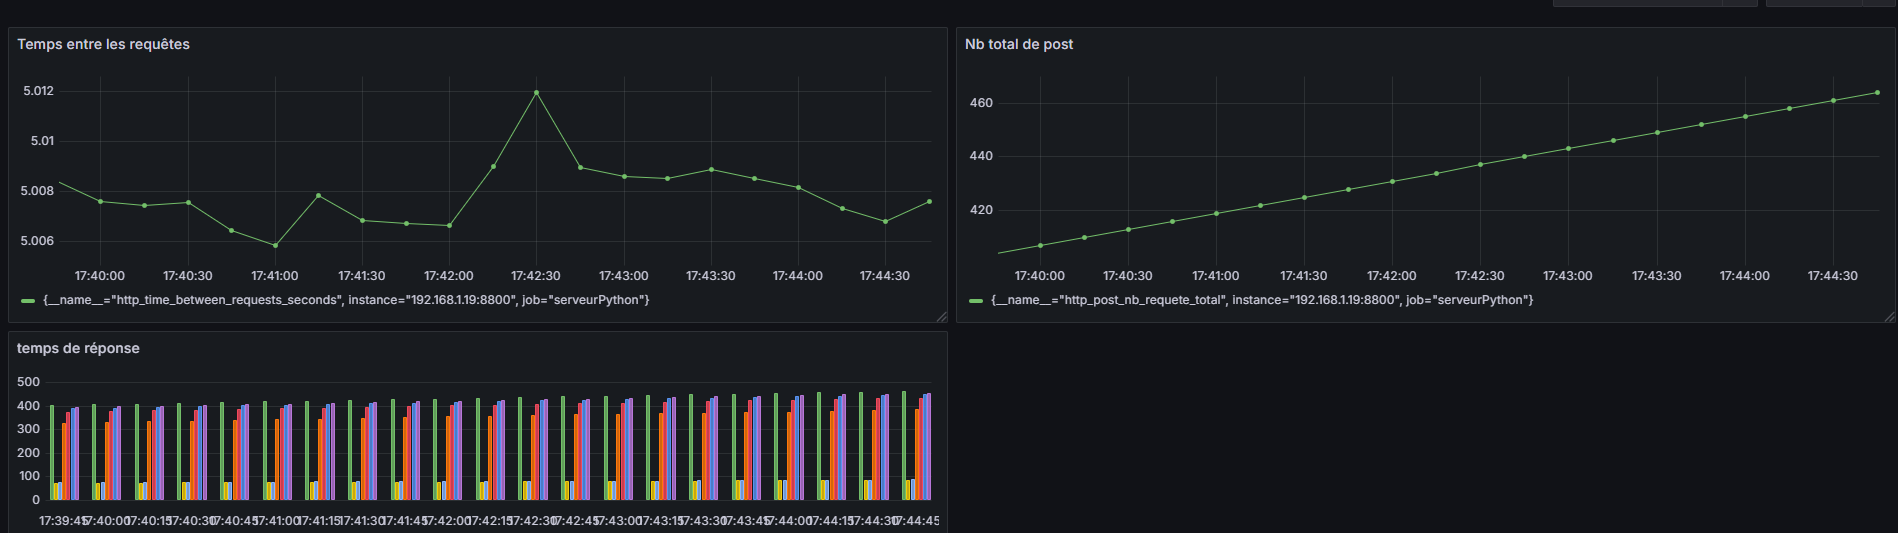
\includegraphics[scale=0.2]{./ressource/exPanel.png}
\end{center}
\end{frame}



\begin{frame}{Technologies proposées (suite)}

\begin{block}{Gestion et surveillance des logs}
\begin{itemize}
\item Loki /grafana
\item Analyse réelle de logs (avec mise en place client VPN)
\end{itemize}
\end{block}

\begin{center}
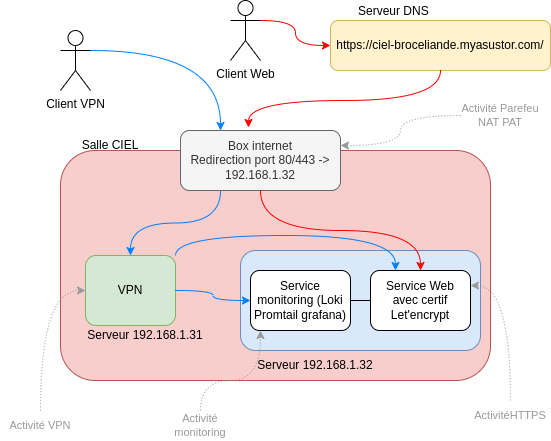
\includegraphics[scale=0.3]{./ressource/topoReseau.drawio.png}
\end{center}
\end{frame}


\begin{frame}{Technologies proposées (suite)}
\begin{block}{Wifi}
\begin{itemize}
\item EBIOS
\item Attaque\textbf{s} / Protection\textbf{s}
\end{itemize}
\end{block}

\begin{center}
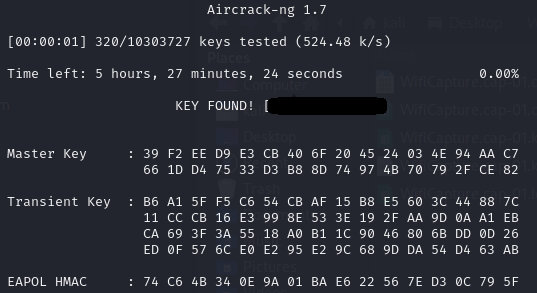
\includegraphics[scale=0.4]{./ressource/clefTrouvee.png}
\end{center}
\end{frame}


\begin{frame}{Technologies proposées (suite)}

\begin{block}{(In)Sécurité du code $\Rightarrow$ Buffer overflow}
\begin{itemize}
\item Bypasser une demande d'authentification avec un buffer overflow
\item Exécuter une fonction normalement non utilisée (plus technique mais fort intéressant). 
\end{itemize}
\end{block}


\begin{center}
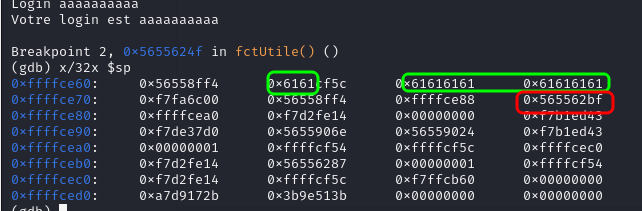
\includegraphics[scale=0.4]{./ressource/dump_mem.png}
\end{center}

\end{frame}



\begin{frame}{\textbf{Finalité}}
\begin{block}{\Large $\Rightarrow$ Partager des idées d'activités et d'outils}
    \small Mettre en commun des ressources 
\end{block}

\begin{block}{\Large $\Rightarrow$ Proposer des solutions de mutualisation}
    \small Échanger sur des solutions 
\end{block}

\begin{alertblock}{\Large $\Rightarrow$ Ne pas réaliser toutes les activités}
    \small Choisir celles qui vous conviennent
\end{alertblock}
\end{frame}



\begin{frame}{Comment ?}

\begin{block}{Énoncés accessibles sur }
\begin{itemize}
\item \url{https://ciel-broceliande.myasustor.com/}
\end{itemize}
\end{block}

\begin{block}{Identifiants}
\begin{itemize}
\item Login : \textit{formationCyber}
\item Mot de passe : \textit{acRennes!!2025}
\end{itemize}
\end{block}


\begin{center}
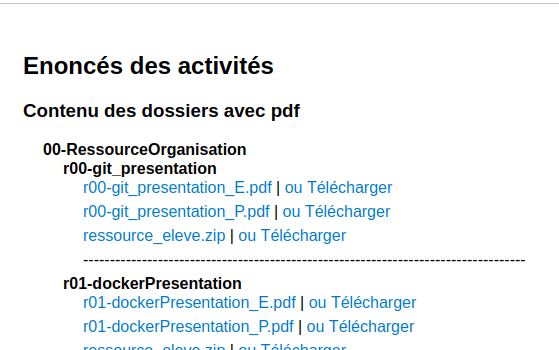
\includegraphics[scale=0.5]{./ressource/enonceSite}
\end{center}

\end{frame}

\begin{frame}{Les dépôts}

\scriptsize % Plus lisible que \tiny
\begin{tabular}{|>{\raggedright\arraybackslash}p{3cm}|
                >{\raggedright\arraybackslash}p{3.5cm}|
                >{\raggedright\arraybackslash}p{4.5cm}|}
\hline
\rowcolor{vert_capet} \textbf{Activités} & \textbf{Description} & \textbf{URL GitHub} \\
\hline

\begin{minipage}{\linewidth}
\vspace{0.2cm}
\begin{itemize}
  \item \texttt{act02-https}
  \item \texttt{act03-monitoring}
  \item \texttt{act04-SNMP\_P}
  \item \texttt{02-wifi}
\end{itemize}\vspace{0.2cm}
\end{minipage}
& Serveur temperature + client python\&ESP32 + falsification client
& \url{https://github.com/PierreViland/serveurSimpleIot.git} \\
\hline

\begin{minipage}{\linewidth}
\begin{itemize}
  \item Toutes
\end{itemize}
\end{minipage}
& Serveur LEMP et LAMP HTTP/HTTPS 
& \url{https://github.com/PierreViland/00-serveurLemp.git} \\
\hline

\begin{minipage}{\linewidth}
\begin{itemize}
  \item \texttt{act02-https}
\end{itemize}
\end{minipage}
& Exemple phishing avec certificat Let's Encrypt 
& \url{https://github.com/PierreViland/httpsPhishingExemple.git} \\
\hline

\begin{minipage}{\linewidth}\vspace{0.2cm}
\begin{itemize}
  \item \texttt{act03-monitoring}
  \item \texttt{act04-SNMP\_P}
  \item \texttt{act05-gestionLog}
\end{itemize}\vspace{0.2cm}
\end{minipage}
& Monitoring stack + Analyse de logs 
& \url{https://github.com/PierreViland/monitoringPV.git} \\
\hline

\begin{minipage}{\linewidth}
\begin{itemize}
  \item \texttt{act04-SNMP\_P}
\end{itemize}
\end{minipage}
& Zabbix 
& \url{https://github.com/akmalovaa/zabbix-docker} \\
\hline

\begin{minipage}{\linewidth}
\begin{itemize}
  \item Bonus
\end{itemize}
\end{minipage}
& Source \LaTeX{} des documents + workflow de déploiement 
& \url{https://github.com/PierreViland/formationCyber2025.git} \\
\hline
\end{tabular}

\normalsize
\end{frame}



\end{document}
